\documentclass{beamer}
\usepackage{graphicx}
\usepackage{blindtext}
\usepackage{natbib}
\mode<presentation> {
\usetheme{Warsaw}
\usecolortheme{crane}}
\title{I social e il populismo}
\author{Alessandro Meloni, Alessandro Casanova}
\date{16/11/2023}

\begin{document}
\maketitle
 
\begin{frame}
    Introduzione autore, pensiero, studi
\end{frame}

\begin{frame}
    Introduzione autore, pensiero, studi
\end{frame}
\begin{frame}
    
\end{frame}
\begin{frame}
\begin{figure}
    \flushleft
    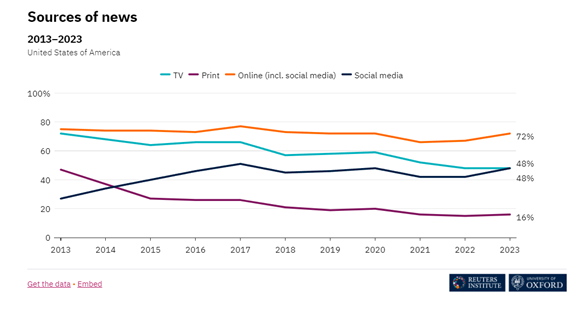
\includegraphics[width=0.6\linewidth]{Sourcesofnews.png}
    \caption{Grafico che spiega l'andamento dell'utilizzo dei diversi media per l'informazione}
    \label{F:graficomezz}
    
\end{figure}
\end{frame}
\begin{frame}
    Populism here becomes a catch-all label to refer to all those political phenomena that are considered to be dangerous, irrational and demagogic; populism as a politics that appeals to the basest sentiments of the populace, makes demagogic promises and panders to imaginary fears.
    \citep{Gerbaudo2018}

\end{frame}
\begin{frame}
\begin{figure}
    \flushleft
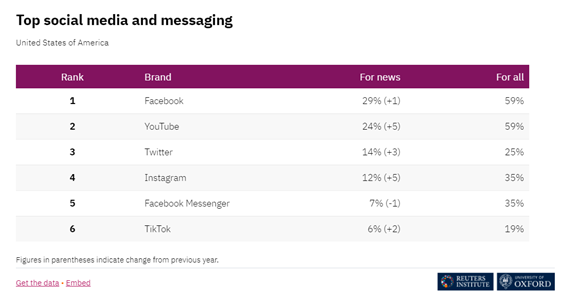
\includegraphics[width=0.6\linewidth]{TopSocial.png}
    \caption{Tabella esplicativa della top 5 social in America}
    \label{F:social}
\end{figure}
\end{frame}
\begin{frame}
    
\end{frame}
\begin{frame}
    
\end{frame}
\begin{frame}
    
\end{frame}
\begin{frame}
    
\end{frame}

\bibliography{Bibliografia}
\bibliographystyle{alpha}
    
\end{document}
